We now consider an elastic solid with square section of dimension $l=3m$ in the ($\vect{e}_1,\vect{e}_2$) plane, and infinite in the direction $\vect{e}_3$ so that the plane strain assumption (\textit{i.e. $\eps_{33}=\eps_{13}=\eps_{23}=0$}) holds. The values of elastic parameters considered are still those of table \ref{tab:material}. The solid suddenly undergoes a tensile stress on a part of its left boundary (see figure \ref{fig:2D_problem}) so that shear and pressure waves travel in the mediumtoward the horizontally fixed right end, reflect and then propagate leftward.
No exact solution is available, comparisons with $Q1$ finite element (bilinear approximation) and MPM solutions are thus performed.
\begin{figure}[h!]
  \centering
  \input{chapter4/pgfFigures/2d_square}
  \caption{Geometry, loading and boundary condition for the tensile impact problem on a two-dimensional elastic medium.}
  \label{fig:2D_problem}
\end{figure}

\begin{figure}[h!]
  \centering
    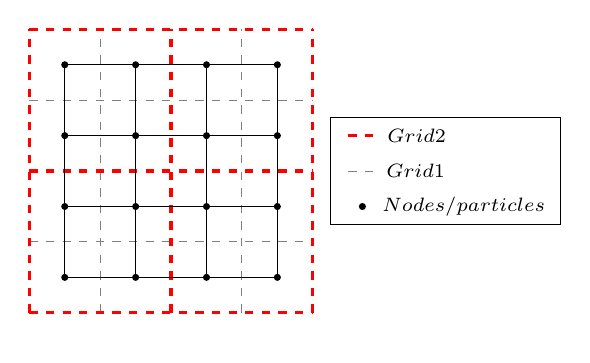
\begin{tikzpicture}[scale=0.9]
  \draw (0,0) --(3,0)--(3,3)--(0,3)--(0,0);
  \draw[white] (0.,0) -- (0,-0.8);
  %%% Grid 1
  \foreach \y in {-0.5,0.5,...,3.5} 
  \draw[dashed,gray] (-0.5,\y) -- (3.5,\y);
  \foreach \x in {-0.5,0.5,...,3.5} 
  \draw[dashed,gray] (\x,-0.5) -- (\x,3.5);
  %%% Grid 2
  \foreach \y in {-0.5,1.5,...,3.5} 
  \draw[dashed,Red,very thick] (-0.5,\y) -- (3.5,\y);
  \foreach \x in {-0.5,1.5,...,3.5} 
  \draw[dashed,Red,very thick] (\x,-0.5) -- (\x,3.5);
  \foreach \y in {0.,1.,...,3.} 
  \foreach \x in {0.,1.,...,3.} 
  \fill (\x,\y) circle(0.05);
  \foreach \y in {0.,1.,...,3.} 
  \draw (0,\y) -- (3.,\y);
  \foreach \x in {0.,1.,...,3.} 
  \draw (\x,0) -- (\x,3);
  \draw (3.75,0.75) rectangle (7.,2.25);
  \fill (4.2,1.) circle (0.05) node [right] {\scriptsize$ \: \: \text{Nodes / particles}$};
  \draw[dashed,gray] (4.,1.5) -- (4.4,1.5) node [right] {\scriptsize$\color{black} \text{Grid 1}$};
  \draw[dashed,very thick,Red] (4.,2.) -- (4.4,2.) node [right] {\scriptsize$\color{black} \text{Grid 2}$};
\end{tikzpicture}


%%% Local Variables:
%%% mode: latex
%%% TeX-master: "../manuscript"
%%% End:

  \caption{Meshes used for the simulations.}
  \label{fig:2d_meshes}
\end{figure}
The solid is discretized such that material points are equivalent to finite element nodes, 
that is $l\times l \equiv 28 \times 28$ particles and nodes. Two arbitrary grids are used for the DGMPM so that either one of four material points lie in every cells as depicted in figure \ref{fig:2d_meshes} for a coarse example.

The finite element computation is performed with the software \textit{Abaqus} \cite{Abaqus}, using an explicit time discretization with no artificial viscosity added . These numerical results are compared to those obtained from DGMPM computations using both CTU and DCU methods. The Courant number is set to unity in DGMPM-CTU and to $0.7$ in DGMPM-DCU leading to \textit{average} time steps $\Delta t_{CTU}=1.57 \times 10^{-5}s$ and $\Delta t_{DCU}=1.13 \times 10^{-5}s$, whereas the \textit{constant} time step used in the FEM simulation is $\Delta t_ {FEM}=1.43 \times 10^{-5} s$. Figure \ref{figure:2D_partial_impact} shows numerical results in terms of the Cauchy stress tensor $\tens{\sigma} = \frac{1}{J}\tens{\Pi}\tens{F}^T$ exported from Abaqus to Paraview with the code developed in \cite{Export_Abaqus}. 


\begin{figure}[h!]
  \centering
  

\begin{figure}\centering
  \begin{tikzpicture}
    \begin{groupplot}[group style={group size=3 by 2,
        ylabels at=edge left, yticklabels at=edge left,
        horizontal sep=.5ex,
        vertical sep=2ex,},
      enlargelimits=0,
      xmin=0.,xmax=1., ymin=-0.,ymax=1.
      ,axis on top,scale only axis,xtick=\empty,ytick=\empty,width=0.25\linewidth,
      colorbar style={
        title style={
          font=\scriptsize,
          at={(1,.5)},
          anchor=north west
        },yticklabel style={font=\scriptsize}
      ,at={(current axis.south east)},anchor=south west
      }]
      %% FIRST ROW (time 1 = 3.5e-4s)
      %%% RANGE -1.6e7 -- 2.9e8
      \nextgroupplot[ylabel={$t=3.5\times 10^{-4} \:s.$},title={FEM}]\addplot graphics[xmin=0.,xmax=1., ymin=-0.,ymax=1.] {chapter4/pngFigures/fem_stress_78.png};
      \nextgroupplot[title={DGMPM 1ppc}]\addplot graphics[xmin=-0.,xmax=1., ymin=-0.,ymax=1.] {chapter4/pngFigures/dgmpm1ppc_stress_78.png};
      \nextgroupplot[title={DGMPM 4ppc},
      colorbar,colorbar style={
        title= {$\sigma_{11}\: (GPa)$},
        ytick={-1.6e-2,2.9e-1},
        %yticklabels={0,0.5,1},
      }]
      \addplot[scatter,scatter src=y,mark size=0.pt] coordinates {(0.,-1.6e-2) (0.,2.9e-1)};% Fake extreme values to fix scale
      \addplot graphics[xmin=-0.,xmax=1., ymin=-0.,ymax=1.] {chapter4/pngFigures/dgmpm4ppc_stress_78.png};

      %% SECOND ROW (time 2 =1.e-3s)
      %%% RANGE -2.9e7 -- 3.5e8
      \nextgroupplot[ylabel={$t=1.0\times 10^{-3} \:s.$}]\addplot graphics[xmin=0.,xmax=1., ymin=-0.,ymax=1.] {chapter4/pngFigures/fem_stress_231.png};
      \nextgroupplot[]\addplot graphics[xmin=-0.,xmax=1., ymin=-0.,ymax=1.] {chapter4/pngFigures/dgmpm1ppc_stress_231.png};
      \nextgroupplot[colorbar,colorbar style={
        title= {$\sigma_{11}\: (GPa)$},
        ytick={-2.9e-2,3.5e-1},
        %yticklabels={0,0.5,1},
      }]
      \addplot[scatter,scatter src=y,mark size=0.pt] coordinates {(0.,-2.9e-2) (0.,3.5e-1)};% Fake extreme values to fix scale
      \addplot graphics[xmin=-0.,xmax=1., ymin=-0.,ymax=1.] {chapter4/pngFigures/dgmpm4ppc_stress_231.png};
      
    \end{groupplot}
  \end{tikzpicture}
  \caption{time $t=3.5e-4s$}
  \label{fig:2delast_comparison1}
\end{figure}



%%% Local Variables:
%%% mode: latex
%%% TeX-master: "../mainManuscript"
%%% End:

  \caption{Longitudinal stress $\sigma_{11}$ isovalues in a linear elastic plate.}
  \label{fig:2delast_comparison1}
\end{figure}



%%% Local Variables:
%%% mode: latex
%%% TeX-master: "../mainManuscript"
%%% End:
